\section{MPI One-Sided Communication}
\subsection{Required submission files}
\begin{enumerate}
	\item \hl{The updated \emph{gauss.c} file.}

		\verb!Data/path/to/file!

	\item \hl{The new performance plots and description in the report.}

		References to figures here...

\end{enumerate}

\subsection{Questions}
\begin{enumerate}
	\item \hl{Which one-sided operations were used? Justify your choice.}

	Answer...

	\item \hl{Was communication and computation overlap achieved? Use Vampir.}

	Answer...

	\item \hl{Was a speedup observed versus the baseline for the Sandy Bridge and Haswell nodes?}

	Answer...

	\item \hl{Was a speedup observed versus the non-blocking version for the Sandy Bridge and Haswell nodes?}

	Answer...

\end{enumerate}
% % Figure example
% \begin{figure}[p] % h=here, t=top, b=bottom, p=(extra)page, !=force
%  	\begin{center}
%  		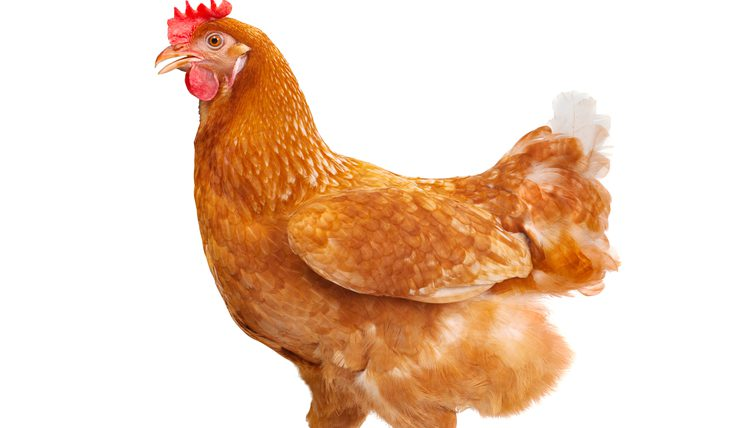
\includegraphics[width=.9\linewidth]{figure.png} % It searches in the Figures/ folder!
%  		\caption{Caption text}
%  		\label{fig:figureLabelName}
%  	\end{center}
% \end{figure}
